\section*{K7/3. feladat: Hőcserélő rendszerek számítása}

\addcontentsline{toc}{section}{K7/3. feladat: Hőcserélő rendszerek számítása}

\begin{tabular}{ | p{2cm} | p{12cm} | } 
	\hline
	Szerző & Lázár Zsolt (AUSFZ6) \\ 
	\hline
	Szak & Vegyészmérnök alapszak \\ 
	\hline
	Félév & 2019/2020 II. (tavaszi) félév \\ 
	\hline
\end{tabular}

\vspace{0.5cm}

\subsection*{Határozza meg a hőcserélő rendszerből kilépő olaj keveredési $ \mathrm{(t_m)}$ hőmérsékletét, a rendszert elhagyó hűtővíz hőmérsékletét $\mathrm{(t_{2vv})}$ és rajzolja le a hőmérséklet-hely függvényt!}

\vspace{1cm}

\flushleft Adatok: \newline \\
\centering
\begin{tabular} [c!] {l l}

$t_{1ok}= \SI{95}{\celsius}$ & $G_{1o}= \SI{20}{\tonne\per\hour}$ \\
$t_{2ok}= \SI{115}{\celsius}$ & $G_{2o}= \SI{30}{\tonne\per\hour}$ \\
$t_{1vk}= \SI{18}{\celsius}$ & $G_{1v}= \SI{18}{\tonne\per\hour}$	\\
$\kappa_1= \SI{500}{watt\per\meter\squared\kelvin}$ & $\kappa_2= \SI{550}{watt\per\meter\squared\kelvin}$ \\
$A_1= \SI{60}{\meter\squared}$ & $A_1= \SI{60}{\meter\squared}$	\\
$c_o= \SI{2,1}{\kilo\joule\per\kilogram\kelvin}$ & $c_v= \SI{4,187}{\kilo\joule\per\kilogram\kelvin}$	\\

\end{tabular}

\vspace{1.5cm}

\begin{figure}[!ht]
\centering
\label{figure:sm}

	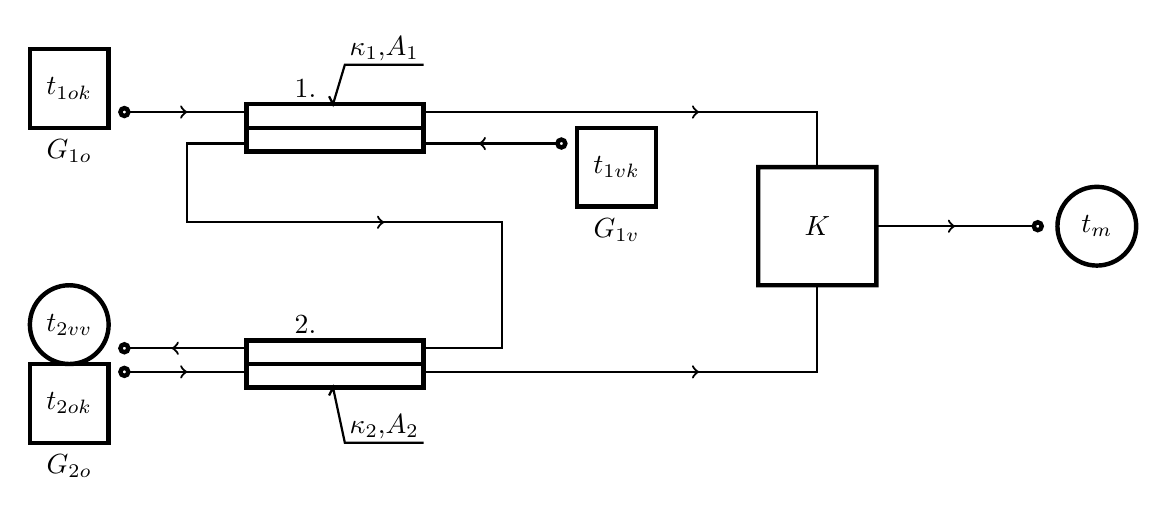
\begin{tikzpicture}

		\draw[ultra thick] (0,0) rectangle (1,1) (0.5,0.5) node{$t_{1ok}$} (0.5,-0.3) node{$G_{1o}$};
		\draw[ultra thick] (1.2,0.2) circle (0.05);
		\draw[thick] (1.25,0.2) -- (2.75,0.2);
		\draw[->, thick] (1.5,0.2) -- (2,0.2);
		\draw[ultra thick] (2.75,0.3) rectangle (5,0) (2.75,0) rectangle (5,-0.3);
		\draw[ultra thick] (3.5,0.5) node{$1.$};
		\draw[thick] (3.8,0.4) -- (3.85,0.3) -- (4,0.8) -- (5,0.8) (4.5,1) node{$\kappa_1$,$A_1$};

		\draw[thick](5,0.2) -- (10,0.2) -- (10,-0.5);
		\draw[ultra thick] (9.25,-0.5) rectangle (10.75,-2) (10,-1.25) node{$K$} (13.55,-1.25) circle (0.5) (13.55,-1.25) node{$t_m$}; 
		\draw[thick] (10.75,-1.25) -- (12.75,-1.25);
		\draw[ultra thick] (12.80,-1.25) circle (0.05);
		\draw[->, thick] (8,0.2) -- (8.5,0.2);
		\draw[->, thick] (11.25,-1.25) -- (11.75,-1.25);

		\draw[ultra thick] (0.5,-2.5) circle (0.5) (0.5,-2.5) node{$t_{2vv}$};
		\draw[ultra thick] (0,-3) rectangle (1,-4) (0.5,-3.5) node{$t_{2ok}$} (0.5,-4.3) node{$G_{2o}$};
		\draw[ultra thick] (1.2,-2.8) circle (0.05);
		\draw[ultra thick] (1.2,-3.1) circle (0.05);

		\draw[thick] (2.75,-0.2) -- (2,-0.2) -- (2,-1.2) -- (6,-1.2) -- (6,-2.8) -- (5,-2.8);
		\draw[->, thick] (4,-1.2) -- (4.5,-1.2);
		\draw[ultra thick] (6.75,-0.2) circle (0.05);
		\draw[thick] (5,-0.2) -- (6.7,-0.2);
		\draw[<-, thick] (5.7,-0.2) -- (6.2,-0.2);
		\draw[ultra thick] (6.95,0) rectangle (7.95,-1) (7.45,-0.5) node{$t_{1vk}$} (7.45,-1.3) node{$G_{1v}$};

		\draw[ultra thick] (2.75,-2.7) rectangle (5,-3) (2.75,-3) rectangle (5,-3.3) (3.5,-2.5) node{$2.$};
		\draw[thick] (3.8,-3.4) -- (3.85,-3.3) -- (4,-4) -- (5,-4) (4.5,-3.8) node{$\kappa_2$,$A_2$};
		\draw[thick] (1.25,-2.8) -- (2.75,-2.8);
		\draw[<-, thick] (1.8,-2.8) -- (2.3,-2.8);
		\draw[thick] (1.25,-3.1) -- (2.75,-3.1) (5,-3.1) -- (10,-3.1) -- (10,-2);
		\draw[->, thick] (8,-3.1) -- (8.5,-3.1); 
		\draw[->, thick] (1.5,-3.1) -- (2,-3.1);
	\end{tikzpicture}
	\caption{A hőcserélő rendszer vázlata}
\end{figure}

\pagebreak

\begin{flushleft}
\subsubsection{a) Írja fel a hőcserélő rendszerre érvényes vektor-mátrix szorzatot és jelölje meg ezek egymással való kapcsolatát!}

\noindent A hőcserélő rendszerben mind a két hőcserélő ellenáramú, és mindkét berendezésben olaj hűtése történik vízzel. Az első hőcserélőből kilépő vízzel hűtjük a második hőcserélőbe belépő olajat. A számolások megkezdése előtt átváltottam az adatokat az SI mértékegységrendszer szerint használatos mértékegységekre.
\end{flushleft}

\flushleft Tömegáram: \newline 
\begin{equation*}
		G_{1o}= \SI{20}{\tonne\per\hour} = \SI{5.56}{\kilogram\per\sec}; \hspace{10pt} 
		G_{2o}= \SI{30}{\tonne\per\hour} = \SI{8.33}{\kilogram\per\sec}; \hspace{10pt}
		G_{1v}= \SI{18}{\tonne\per\hour} = \SI{5.00}{\kilogram\per\sec};
\end{equation*}
\flushleft Fajhő: \newline
\begin{equation*}
		c_o= \SI{2,1}{\kilo\joule\per\kilogram\kelvin} = \SI{2100}{\joule\per\kilogram\kelvin}; \hspace{15pt}
		c_v= \SI{4,187}{\kilo\joule\per\kilogram\kelvin} = \SI{4187}{\joule\per\kilogram\kelvin};
\end{equation*}
\vspace{5pt}



Az első hőcserélőből kilépő olaj ($t_{11k}$) és a víz ($t_{11kv}$) hőmérsékletét, valamint a második hőcserélőből kilépő olaj ($t_{22k}$) és víz ($t_{2vv}$) hőmérsékletét kell meghatározni, ezért két független egyenletet kell felírnunk. Az egyes hőcserélőkben a leadott, az átszármaztatott és a felvett hőáram az energiamegmaradás miatt egyenlő. A leadott és a felvett hőáram egyenlőségéből a véghőmérsékletekre lineáris egyenletet kapunk, az átszármaztatott hőáram viszont csak akkor ad lineáris egyenletet, ha a konvektív vízértékek egyenlők. A kiszámolt konvektív vízértékek:
\begin{equation*}
		w_{1o} = G_{1o} c_o = \SI{11676}{\watt\per\kelvin}; \hspace{10pt} 
		w_{2o} = G_{2o} c_o = \SI{17493}{\watt\per\kelvin}; \hspace{10pt}
		w_{1v} = G_{1v} c_v = \SI{20935}{\watt\per\kelvin};
\end{equation*}
Láthatjuk, hogy a konvektív vízértékek nem egyenlőek, ezért szükséges keresni egy olyan egyenletet ami lineáris. Ez lehet a $\Delta t(A)$ hőmérséklet-hely függvény teljes $A$ hőátadó felületre.
\begin{equation}
	\Delta t(A) = \Delta t_N \mathrm{e}^{-\kappa m A} = \Delta t_K
\end{equation}
A $\Delta t_N$ és a $\Delta t_K$ hőmérséklet-különbségek helyes felírására kell odafigyelni, mivel ellenáramú hőcserélőnél a nagyobb konvektív vízértékű közeg belépésénél lesz a kisebb hőmérséklet-különbség, esetünkben az első hőcserélőnél $\Delta t_N = t_{1ok}-t_{11vk}$ az olaj belépésénél és $\Delta t_K = t_{11k}-t_{1vk}$ a víz belépésénél, így a két ismeretlen véghőmérsékletre az alábbi kétismeretlenes egyenletrendszert tudjuk felírni:
\begin{gather*}
	I.\: -w_{1o} (t_{11k} - t_{1ok}) = w_{1v} (t_{11vk} - t_{1vk}) \\
	II.\: (t_{1ok} - t_{11vk})\mathrm{e}^{-\kappa_1 m_1 A_1} = t_{11k} - t_{1vk}
\end{gather*}

Az egyenletek paraméteres rendezése után a két ismeretlent $\mat{t_v} = c \mat{A} \mat{t_k}$, mátrixos alakba írhatjuk fel.

Az olaj kilépési hőmérséklete:
\begin{equation*}
		t_{11k} = \dfrac{1}{1-\eta \varphi} 
	\begin{bmatrix}
		\eta (1- \varphi) & 1-\eta
	\end{bmatrix} 
	\begin{bmatrix}
		t_{1ok} \\
		t_{1vk}
	\end{bmatrix}
\end{equation*}
A víz kilépési hőmérséklete:
\begin{equation*}
		t_{11vk} = \dfrac{1}{1-\eta \varphi}
	\begin{bmatrix}
		\varphi(1-\eta) & 1-\varphi
	\end{bmatrix} 
	\begin{bmatrix}
		t_{1ok} \\
		t_{1vk}
	\end{bmatrix}
\end{equation*}

\pagebreak

A két ismeretlen mátrixos alakját összevonva és a lineáris kombinációjukat képezve megkaphatjuk az első hőcserélőből kilépő hőmérsékleteket:
\begin{equation*}
	\begin{bmatrix}
		{t_{11k}} \\
		{t_{11vk}}
	\end{bmatrix}
	=
	\dfrac{1}{1 - \eta \varphi}
	\begin{bmatrix}
		\eta(1-\varphi) & 1-\eta \\
		\varphi(1-\eta) & 1-\varphi
	\end{bmatrix}
	\begin{bmatrix}
		t_{1ok} \\
		t_{1vk}
	\end{bmatrix}
\end{equation*}
\noindent Ugyanezen összefüggések érvényesek a másik hőcserélőre is, így fel tudjuk arra is írni az ismeretlen kilépő hőmérsékletekre felállított mátrixos alakot.
\subsubsection{b) Számítsa ki a hőcserélőkre vonatkozó $\varphi$ és $\eta$ értékeket, majd a kilépési hőmérsékletet!} 
\noindent Az első hőcserélő esetében a számolt $\varphi$, $\eta$ és $m$ értékek:
\begin{gather*}
		\varphi_1 = \dfrac{w_{1o}}{w_{1v}} = \SI{0.56}{}; \\ 
		\eta_1 = \mathrm{e}^{-\kappa_1\cdot m_1\cdot A_1} = \SI{0.32}{}; \\
		m_1 = \dfrac{1}{w_{1o}}-\dfrac{1}{w_{1v}} = \SI{3.79e-5}{\kelvin\per\watt};
\end{gather*}
\noindent A második hőcserélő esetében számolt $\varphi$, $\eta$ és $m$ értékek:
\begin{gather*}
		\varphi_2 = \dfrac{w_{2o}}{w_{1v}} = \SI{0.84}{}; \\ 
		\eta_2 = \mathrm{e}^{-\kappa_2\cdot m_2\cdot A_2} = \SI{0.73}{}; \\
		m_2 = \dfrac{1}{w_{2o}}-\dfrac{1}{w_{1v}} = \SI{9.4e-6}{\kelvin\per\watt};
\end{gather*}
\noindent Az $\eta$ az exponenciális függvény értéke, a $\varphi$ a konvektív vízértékek hányadosa, az $m$ pedig a konvektív vízértékek reciprokainak különbsége.

\vspace{10pt}
A számolások nagy részét MATLAB-ban végeztem el, az adatok és a mátrixos forma helyes bevitele után, így az első, illetve a második hőcserélőből kilépő olaj és víz hőmérsékletére az alábbi eredményeket kaptam:
\vspace{10pt} \newline
Első hőcserélő: 
\begin{equation*}
	t_{11k} = \SI{31.31}{\celsius}; \hspace{15pt}
	t_{11vk} = \SI{53.52}{\celsius};
\end{equation*}

Második hőcserélő:
\begin{equation*}
	t_{22k} = \SI{78.71}{\celsius}; \hspace{15pt}
	t_{2vv} = \SI{92.63}{\celsius};
\end{equation*}

\subsubsection{c) Írja fel a keverőfejre a keveredési hőmérsékletet (keveredési hőt itt nem vesszük figyelembe)!}
\noindent A keverési egyenlettel számoltam ki, hogy mennyi lesz az olaj végső hőmérséklete:
\begin{equation*}
		t_m = \dfrac{(G_{1o}\cdot t_{11k})+(G_{2o}\cdot t_{22k})}{(G_{1o}+G_{2o})} = \SI{59.74}{\celsius}
\end{equation*}

\subsubsection{d) Rajzolja le a hőcserélők hőmérséklet-hely függvényét!}
